\documentclass[12pt,a4paper]{ctexart}

\usepackage[UTF8]{ctex}
\usepackage{geometry}
\usepackage{graphicx}
\usepackage{xcolor}
\usepackage{tikz}
\usepackage{fontspec}
\usepackage{setspace}
\usepackage{enumitem}
\usepackage{booktabs}
\usepackage{array}
\usepackage{longtable}
\usepackage{hyperref}
\usepackage{fancyhdr}
\usepackage{titlesec}
\usepackage{multicol}
\usepackage{xurl}
\usepackage{tocloft}

\renewcommand{\cfttoctitlefont}{\hfill\bfseries\Large}
\renewcommand{\cftaftertoctitle}{\hfill}
\geometry{left=2.5cm,right=2.5cm,top=2.5cm,bottom=2.5cm}

\definecolor{black}{RGB}{0,0,0}
\definecolor{mainblue}{RGB}{0,82,147}
\definecolor{accentgold}{RGB}{180,140,60}
\definecolor{lightgray}{RGB}{245,245,245}
\definecolor{darkgray}{RGB}{80,80,80}
\definecolor{mainred}{RGB}{230,1,45}

\hypersetup{
    colorlinks=true,
    linkcolor=black,
    urlcolor=mainblue,
    citecolor=mainblue,
    pdfborder={0 0 0}
}

\pagestyle{fancy}
\fancyhf{}
\fancyhead[L]{\small\color{darkgray}\textbf{量子行业每周新闻洞察}}
\fancyhead[R]{\small\color{darkgray}\textbf{总第190期}}
\fancyfoot[C]{\thepage}
\renewcommand{\headrulewidth}{0.4pt}
\renewcommand{\footrulewidth}{0pt}

\titleformat{\section}
    {\Large\bfseries\color{mainred}}
    {\thesection、}{0em}{}
\titleformat{\subsection}
    {\large\bfseries\color{mainred}}
    {\thesubsection、}{0em}{}

\newcolumntype{L}[1]{>{\raggedright\arraybackslash}p{#1}}
\newcolumntype{C}[1]{>{\centering\arraybackslash}p{#1}}

\begin{document}

% ==================== 封面 ====================
\begin{titlepage}
\begin{tikzpicture}[remember picture,overlay]
    \fill[mainred] ([yshift=-0.5cm]current page.north west) rectangle ([yshift=-1.2cm]current page.north east);
    \fill[mainred] ([yshift=1.2cm]current page.south west) rectangle ([yshift=0.5cm]current page.south east);
\end{tikzpicture}

\vspace*{4cm}

\begin{center}
    {\fontsize{44}{52}\selectfont\bfseries\color{black} \textbf{量子行业每周新闻洞察}}

    \vspace{0.8cm}

    {\fontsize{16}{22}\selectfont\color{darkgray} 2026.07.25 — 2026.07.31 }
    {\fontsize{16}{22}\selectfont\color{darkgray} \textbf{WEEKLY NEWS}}

    \vspace{1.5cm}

    {\fontsize{20}{26}\selectfont\color{mainred}\textbf{（总第\textbf{ 190 }期）}}

    \vspace{4cm}

    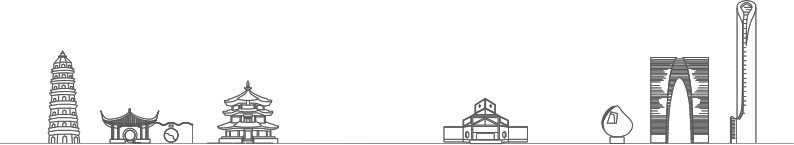
\includegraphics[width=\textwidth]{Cover_Suzhou.png}

    \vfill

    {\fontsize{12}{16}\selectfont\color{darkgray} 量子科技长三角产业创新中心\\编制：科技委办公室、产业发展部（理事会办公室）}
\end{center}
\end{titlepage}

% ==================== 目录 ====================
\pagenumbering{roman}
\newpage
\tableofcontents

\newpage

% ==================== 摘要 ====================
\pagenumbering{arabic}
\setcounter{page}{1}
\begin{center}
{\Large\bfseries\color{mainred} 摘\hspace{2em}要}
\end{center}
\addcontentsline{toc}{section}{摘要}


\textbf{ 宏观态势：}

全球量子技术正加速从实验室走向国家战略与产业基础设施层面。欧美在量子网络布局上持续领跑，从美国开放接入的纠缠量子网络ABQ-Net到卢森堡EuroHPC量子计算机建设，均体现出政府与产业界的深度协同。值得关注的是，量子安全正成为金融、通信等关键行业的当务之急，英国NCSC与香港金管局的行动表明监管机构已开始系统性推动后量子密码迁移。此外，量子教育与劳动力培训、北约等防务组织对量子技术的兴趣，均显示出生态建设的多元化趋势。


\textbf{ 科技前沿：}

科研焦点集中于提升量子系统的可扩展性与纠错能力，并探索新材料、新架构以突破现有技术瓶颈。从金刚石色心单光子源、镱-171亚稳态架构到新型超导量子架构，各方都在努力解决量子比特相干性与错误率这一核心难题。同时，量子技术开始向传感、通信等应用场景渗透，例如低功耗金刚石磁力计用于生物磁场探测、芯片间声学量子信息传输等，表明前沿研究正朝着可集成、低功耗、贴近实际应用的方向演进。


\textbf{ 产品动态：}

后量子密码（PQC）的落地部署明显提速，产品形态从软件算法向硬件信任根、加密态势管理平台等综合解决方案延伸，显示出企业正为“量子威胁日”提前构建系统性防线。与此同时，量子技术产品开始与AI深度融合，例如韩国Norma探索AI智能体驱动量子计算工作流，以及SEALSQ面向物理AI打造量子安全硬件，预示着“量子+AI”有望成为下一代技术融合的重要方向。


\textbf{ 企业资讯：}

产业链上下游合作空前活跃，量子计算正从单一硬件研发向“硬件—软件—应用—生态”全栈式协同发展。IonQ收购SkyWater强化芯片制造能力，反映了垂直整合趋势；而Horizon Quantum与QM、Rigetti与HPE等合作则聚焦于硬件与算法的联合优化。值得关注的是，量子纠错开源生态（如DeltaKit社区基金）、跨国研发合作以及针对物流、通信等垂直行业的应用探索，都表明企业正加速将量子技术转化为商业价值。


\textbf{ 资本运作：}

量子计算赛道正迎来资本市场的强烈追捧，两笔大额融资均来自欧洲企业，反映出该地区量子生态的崛起。Multiverse Computing以5.7亿美元C轮融资和17亿美元估值高居榜首，其B轮到C轮间估值5倍的增长，或体现了市场对量子软件与算法商业化前景的重新评估。ZuriQ在种子轮即获2500万美元，也显示出资本对早期量子初创企业的出手愈发果断和慷慨。




\textbf{ 专利动态：}

本周专利动态涵盖低温环境系统、超导量子测控技术、量子软件与算法、量子算力网共4个板块、16条专利。




% ==================== 会议列表 ====================
{
    \newpage
    \section*{ 8月量子科技行业国内、国际会议}
    \addcontentsline{toc}{section}{ 8月量子科技行业国内、国际会议}
    \scriptsize
    \begin{longtable}{C{0.8cm}L{2.5cm}L{3cm}L{7cm}}
        \toprule[1.5pt]
        \textbf{序号} & \textbf{日期} & \textbf{地点} & \textbf{会议名称} \\
        \midrule
        \endfirsthead
        \toprule
        \textbf{序号} & \textbf{日期} & \textbf{地点} & \textbf{会议名称} \\
        \midrule
        \endhead
        \bottomrule
        \endfoot
        
        1 & 8月3日-5日 & 博尔德及线上, 美国 & 天气与气候应用的量子计算与传感研讨会 \\
        \midrule[0.05pt]
        
        2 & 8月3日-14日 & 贝纳斯克, 西班牙 & 容错量子技术研讨会 \\
        \midrule[0.05pt]
        
        3 & 8月7日-9日 & 杭州, 中国 & 第2届量子计算与通信技术国际会议（ICQCT 2026） \\
        \midrule[0.05pt]
        
        4 & 8月10日-14日 & 纳塔尔, 巴西 & 量子热力学会议2026（QTD 2026） \\
        \midrule[0.05pt]
        
        5 & 8月10日-14日 & 阿姆斯特丹, 荷兰 & QSim2026 \\
        \midrule[0.05pt]
        
        6 & 8月14日-16日 & 印第安纳波利斯, 美国 & 量子AI与自然语言处理2026会议（QNLPAI 2026） \\
        \midrule[0.05pt]
        
        7 & 8月16日-21日 & 巴德洪内夫, 德国 & 量子机器学习暑期学校（Bad Honnef物理学校） \\
        \midrule[0.05pt]
        
        8 & 8月16日-22日 & 贝纳斯克, 西班牙 & 悬浮系统量子工程研讨会 \\
        \midrule[0.05pt]
        
        9 & 8月17日-21日 & 多伦多, 加拿大 & 第11届量子信息与量子控制会议（CQIQC-XI） \\
        \midrule[0.05pt]
        
        10 & 8月17日-21日 & 阿姆斯特丹, 荷兰 & 第23届量子物理与逻辑国际会议（QPL 2026） \\
        \midrule[0.05pt]
        
        11 & 8月24日-28日 & 渥太华, 加拿大 & QCrypt 2026 \\
        \midrule[0.05pt]
        
        12 & 8月24日-28日 & 大田, 韩国 & 第26届亚洲量子信息科学会议 (AQIS) \\
        \midrule[0.05pt]
        
        13 & 8月24日-28日 & 维也纳, 奥地利 & 第9届青年量子信息科学家国际会议 (YQIS) \\
        \midrule[0.05pt]
        
        14 & 8月25日-28日 & 哥德堡, 瑞典 & 超导量子比特与算法 2026 (SQA) \\
        \midrule[0.05pt]
        
        15 & 8月30日-9月1日 & 布雷钦, 英国 & 量子ARC写作静修 \\
        \midrule[0.05pt]
        
        16 & 8月31日-9月3日 & 仁川, 韩国 & 硅量子电子学研讨会 2026 (SiQEW) \\
        \midrule[0.05pt]
        
        17 & 8月31日-9月3日 & 泰恩河畔纽卡斯尔, 英国 & Photon 2026 \\
        \midrule[0.05pt]
        
        18 & 8月31日-9月4日 & 瓦莱塔, 马耳他 & Qalypso 2026暑期学校—量子优化技术与计算物理 \\
        \midrule[0.05pt]
        
        19 & 8月31日-9月4日 & 舍布鲁克, 加拿大 & 量子计算、通信与密码学理论 2026 (TQC) \\
        \midrule[0.05pt]
        
        20 & 8月31日-9月10日 & 格但斯克, 波兰 & Q-Camp: 量子暑期学校 2026 \\
        \midrule[0.05pt]
        
    \end{longtable}
}




% ==================== 宏观态势 ====================
\newpage
\section{宏观态势}
\vspace{-0.5em}
\noindent\rule{\linewidth}{1.5pt}

\subsection{ 美国量子经济发展联盟发布新版《量子网络应用路线图》 }

2026年07月30日消息，美国量子经济发展联盟（QED-C）发布新版《量子网络应用路线图》，确定安全通信、网络计算和分布式传感等领域10个应用，包括量子密钥分发、盲量子计算、集群式和分布式量子计算及分布式量子传感。路线图指出，量子光网络交换机、量子中继器和量子卫星基础设施是多数应用的必要条件，量子光源与光-物质界面技术进步对众多应用至关重要。目前，现有量子网络性能仅支持量子密钥分发和分布式量子传感，且限于点对点短距离部署。

\noindent\textbf{报道链接：}\url{https://www.hpcwire.com/off-the-wire/qed-c-roadmap-identifies-infrastructure-priorities-critical-to-scaling-quantum-networks/}

\subsection{ 量子技术公司Qubitrium宣布参与北约双重用途量子技术暑期培训计划 }

2026年07月29日消息，量子技术公司Qubitrium宣布，将作为共同组织者和学术联合主任参与北约科技组织（NATO STO）2026年暑期培训计划“双重用途量子技术”。该项目由加泰罗尼亚电信技术中心、北约通信与信息局、代尔夫特理工大学、卡尔斯鲁厄理工学院及NATO STO联合举办，面向北约北约成员国及伙伴国的研究生、早期研究人员、行业专家和政策制定者，旨在教育在科学、安全和创新交叉领域工作的下一代量子专业人员。

\noindent\textbf{报道链接：}\url{https://qbn.world/qubitrium-contributes-to-the-nato-sto-summer-training-programme-on-dual-use-quantum-technologies/}

\subsection{ 英国NCSC与沃达丰联合发布后量子密码迁移建议，敦促组织提前应对量子威胁 }

2026年07月29日消息，英国国家网络安全中心（NCSC）与沃达丰（Vodafone）分享了双方联合主办的英国首次政府与行业后量子密码（PQC）迁移专题研讨会形成的关键建议，旨在帮助各类机构为迈向量子安全未来做好准备。该建议指出，未来足够强大的量子计算机将能破解当前保护网络与系统的公钥密码体系体系，因此相关系统必须迁移至可同时抵御量子计算机和经典计算机攻击的PQC算法。去年，NCSC已发布PQC迁移关键时间节点，敦促机构立即行动。NCSC强调，PQC迁移不仅是技术挑战，更是关乎工业界与政府整体韧性的全球战略优先事项。

\noindent\textbf{报道链接：}\url{https://www.vodafone.com/news/newsroom/technology/the-national-cyber-security-centre-and-vodafone-highlight-importance-of-collaboration-in-post-quantum-cryptography-migration}

\subsection{ 香港金管局发布《香港银行业量子准备度白皮书》，并公布量子准备度指数 }

2026年07月29日消息，香港金管局发布《香港银行业量子准备度白皮书》，首次公布量子准备度指数，评分仅2.3分（满分10分），显示银行业量子技术部署处于初步阶段。约68\%受访银行已具备认知或进入规划与试行阶段，32\%尚未启动过渡。后量子密码学方面，约半数银行尚未制定正式规划，半数已在董事会层面讨论量子计算应用，三分之一已探索或试行相关技术。金管局将通过实务指引、技能培训和业界交流，支持银行业2030年前做好准备，并开发后量子密码学工具。

\noindent\textbf{报道链接：}\url{https://www.hkma.gov.hk/chi/news-and-media/press-releases/2026/07/20260727-3/}

\subsection{ Bloq Quantum与QClairvoyance达成合作，共推量子教育与劳动力培训 }

2026年07月29日消息，量子软件基础设施提供商Bloq Quantum与量子技术研究与教育机构QClairvoyance宣布建立战略合作伙伴关系，双方将共同推动量子教育、劳动力培训及机构应用推广，加速量子计算的普及。根据协议，QClairvoyance将作为量子技能合作伙伴，把 Bloq Q Quantum 的平台整合到其培训课程、认证计划及学术合作项目中。此外，双方还将探索联合研究、学术出版、资助申请等合作方向，并计划未来将QClairvoyance的算法集成至Bloq Quantum的平台。

\noindent\textbf{报道链接：}\url{http://www.qtc.com.cn/flash/178529344538108.html}

\subsection{ 四家量子技术企业签约加入美国首个开放接入的纠缠量子网络ABQ-Net }

2026年07月29日消息，四家量子企业Infleqtion、Bandelier、Tensora与Aliro签约加入美国首个开放接入、基于纠缠的量子网络ABQ-Net。该网络位于新墨西哥州，由Qunnect建设，属该州超4.5亿美元量子企业投资计划一部分。Infleqtion将探索原子钟与纠缠粒子实现网络时间同步；Tensora研究量子启发传感检测细微地质变化；Bandelier探究量子纠缠与新型AI模型提升国防及关键基础设施网络韧性；Aliro基于Qunnect纠缠分发系统演示AlirOS KeyGen栈，实现实时纠缠基安全密钥生成。

\noindent\textbf{报道链接：}\url{https://www.qunnect.inc/press-releases/2026-07-28}

\subsection{ 田纳西州量子黑客松将于11月在查塔努加举办，将利用量子技术探索能源领域复杂挑战 }

2026年07月28日消息，由The Company Lab联合查塔努加量子协作组织（CQC）与田纳西大学查塔努加分校合作举办的田纳西量子黑客松现已开放报名。这场36小时创新挑战赛将于11月13日至15日在美国查塔努加举行，届时来自不同学科的大学生将组成团队，共同探索量子技术如何帮助解决电力行业面临的复杂挑战。结合田纳西州在能源、量子研究、基础设施、先进计算及创业方面的优势，主办方希望借助该活动发掘新兴人才，探索该州能源领域如何释放部分潜力。

\noindent\textbf{报道链接：}\url{https://www.prnewswire.com/news-releases/chattanooga-to-host-tennessee-quantum-hackathon-302835474.html}

\subsection{ EuroHPC JU将在卢森堡建量子计算机MeluXina-Q，预算达1195万欧元 }

2026年07月27日消息，欧洲高性能计算联合体（EuroHPC JU）启动采购流程，在卢森堡建设EuroHPC量子计算机，由LuxProvide托管运营，集成至现有超算系统MeluXina中。系统名MeluXina-Q，初期配备至少10个半导体自体自旋量子比特QPU，计划逐步升级至超80个物理量子比特，支持经典-量子混合工作流。总采购预算1195万欧元，由EuroHPC JU与卢森堡政府各承担50\%。

\noindent\textbf{报道链接：}\url{https://www.eurohpc-ju.europa.eu/eurohpc-ju-launches-procurement-quantum-computer-luxembourg-2026-07-23\_en}


% ==================== 科技前沿 ====================
\newpage
\section{科技前沿}
\vspace{-0.5em}
\noindent\rule{\linewidth}{1.5pt}

\subsection{ 美国联合量子研究所科研人员探索量子计算机及其错误如何增强人工智能 }

2026年07月28日消息，美国联合量子研究所（JQI）的研究人员与合作者在《物理评论快报》上发表一篇论文，探讨量子计算如何影响与增强人工智能。该团队在多种量子计算平台上运行神经网络实验，结果表明，源自测量的有意量子随机性对神经网络具有积极作用。他们还观察到，当前量子计算机中普遍存在的错误可能在能在运行神经网络时发挥有益作用。实验中，研究人员针对一个神经网络原本无法正确识别的特定图像进行反复测试，在添加最优随机性后，基于离子阱的量子计算机几乎总能正确识别该数字，而IBM的量子计算机成功率也达到了约90\%。这一发现为利用量子计算固有特性提升AI性能提供了新思路。

\noindent\textbf{报道链接：}\url{https://www.umdphysics.umd.edu/about-us/news/research-news/2113-ai-quantum.html}

\subsection{ 科学家提出新型声学概念，有望实现单个芯片间进行远距离量子信息传输 }

2026年07月28日消息，英国华威大学的研究人员与合作者提出一种“量子声子链接”的新概念，有望实现单个芯片上大量量子比特间的远距离通信。该方法利用一种名为“压缩应变锗硅”（cs-GoS）的特制材料，使量子比特对穿过薄锗晶层的微小振动高度敏感。通过精确工程化控制这些振动，研究团队证明，量子信息原则上可以在相邻或相距整个半导体芯片（直径可达300毫米）的量子比特间进行传输。这一概念为跨芯片量子通信提供了全新的声学路径，有望推动可扩展量子计算架构的发展。相关成果已发表在近日的《APL Quantum》期刊上。

\noindent\textbf{报道链接：}\url{https://www.eurekalert.org/news-releases/1137704}

\subsection{ 伊利诺伊大学研究团队利用新型金刚石色心IL1造出单光子量子源 }

2026年07月28日消息，美国伊利诺伊大学厄巴纳-香槟分校的研究人员在金刚石中发现了一种可作为量子光发射器的新型色心，并将其命名为IL1。该发射器能够发射异常明亮且窄带宽的量子光，由单光子组成，同时对金刚石晶格中常见的晶体振动具有显著的不敏感性。与传统发射器不同，IL1不与大量体晶体振动耦合，而是与单一、可控的局域振动耦合。这种特定振动不会显著破坏发光特性，反而有望被调控并作为一种新型量子资源加以利用。相关研究成果已于日前发表在《自然通讯》上。

\noindent\textbf{报道链接：}\url{https://ece.illinois.edu/news/new-diamond-quantum-emitter-with-potential-to-advance-quantum-technologies}

\subsection{ 长春光机所研究团队提出新型量子级联激光器，可实现室温低功耗激光发射 }

2026年07月28日消息，中国科学院长春光学精密机械与物理研究所孟博研究员团队提出一种采用高脚杯形波导结构的新型量子级联激光器（QCL），实现了室温低功耗激光发射。在该研究中，团队制备并表征了多种尺寸的高脚杯QCL器件，其中1mm × 3μm尺寸的器件在室温（293 K）下连续波阈值功耗约为1W，脉冲阈值低至0.85W，室温连续波输出功率超过27mW，在低温（243 K）下连续波和脉冲输出功率分别达到83mW和130mW。该设计为降低QCL功耗、推动其在室温下的实用化提供了新路径。相关成果已发表于《Laser \& Photonics Reviews》期刊。

\noindent\textbf{报道链接：}\url{http://english.ciomp.cas.cn/RD/ResearchProgress/202607/t20260727\_1179176.html}

\subsection{ 日本科学家开发出低功耗金刚石量子磁力计，可实现近距离生物磁场探测 }

2026年07月27日消息，日本东京科学大学的一个研究团队开发出一种基于Ramsey干涉技术的低功耗金刚石量子磁力计，可在不牺牲热安全性的前提下实现高灵敏度生物磁场测量。该传感器仅使用210毫瓦的低功率激光，结合光捕获金刚石波导和紧凑型微波天线，在传感器与样品间距仅2毫米时，传感单元温升仅13开3开尔文，成功探测到皮特斯拉级（10⁻¹2T）磁场。该传感器为未来磁心电图和磁脑电图应用提供了安全、近距离的生物磁场测量方案。相关研究成果已于日前发表在《应用物理快报》。

\noindent\textbf{报道链接：}\url{https://www.isct.ac.jp/en/news/c8rn3errkru9}

\subsection{ 普林斯顿大学提出镱-171亚稳态量子计算架构，利用可检测擦除错误提升纠错能力 }

2026年07月27日消息，普林斯顿大学的研究人员提出了一种构建量子计算机的新方法，旨在减少计算错误并提高错误的检测与修正效率。该团队设计的策略是开发一种基于亚稳态镱-171原子的量子计算平台，这种特定同位素的中性原子处于长寿命的激发态。通过精心设计基于亚稳态镱-171原子的量子比特，确保其产生可检测的擦除错误，这种错误能使量子计算系统直接定位“问题”量子比特。为修正这些已识别的错误，团队还提出了一种量子纠错码，仅需四个物理量子比特即可编码两个逻辑量子比特。这一成果有望为构建更稳定、更易于纠错的量子计算系统提供新的实现路径。相关成果已于近日发表在《自然物理》上。

\noindent\textbf{报道链接：}\url{https://phys.org/news/2026-07-quantum-circuits-based-neutral-atoms.html}

\subsection{ 芝加哥大学等团队展示新型超导量子架构，有望推动拓扑量子计算发展 }

2026年07月27日消息，一个由芝加哥大学、普渡大学、波士顿大学及AppliedTQC研究人员组成的团队，通过实验展示了一种新型超导量子电路架构，可在实验中实现此前仅存在于理论模型中的关键规范对称性，为构建未来拓扑量子计算系统提供硬件基础。该器件验证了一种理论架构里的基本构建单元，当组装成更大规模的晶格时，这一架构有望最终支持拓扑保护的量子态。这一成果为构建更稳定、抗退相干能力更强的量子比特提供了实验基础，标志着拓扑量子计算从理论走向物理实现迈出了关键一步。相关研究论文已于近日发表在预印本平台arXiv上。

\noindent\textbf{报道链接：}\url{https://thequantuminsider.com/2026/07/21/researchers-demonstrate-new-superconducting-circuit-design-that-could-advance-topological-quantum-computing/}


% ==================== 产品动态 ====================
\newpage
\section{产品动态}
\vspace{-0.5em}
\noindent\rule{\linewidth}{1.5pt}

\subsection{ 面向物理AI时代，SEALSQ加速推进量子安全的硬件信任根 }

2026年07月30日消息，SEALSQ宣布更新其最初于2026年3月公布的抗量子硬件认证路线图。该公司表示，随着人工智能向自主物理AI系统演进，从机器人、车辆到边缘设备，每台设备都需要通过芯片中的硬件信任根实现身份验证、通信保护、AI模型安全及可信更新，而量子计算正使传统密码学面临失效风险，因，因此设计寿命长达10至20年的产品必须提前具备后量子准备。SEALSQ目前正在向客户提供其TPM185后量子密码可信平台模块样品，该模块基于最新标准化的PQC算法设计，可供客户评估和产品集成，帮助OEM和系统制造商提前构建量子韧性平台。

\noindent\textbf{报道链接：}\url{https://www.globenewswire.com/news-release/2026/07/29/3335213/0/en/Physical-AI-Requires-Quantum-Safe-Chips-Today-SEALSQ-Common-Criteria-Certification-Will-Strengthen-Trust-for-Tomorrow.html}

\subsection{ Cloudflare新动作：两项产品已支持后量子身份认证ML-DSA算法 }

2026年07月30日消息，Cloudflare宣布，其Authenticated Origin Pulls和Custom Origin Trust Store两款产品现已支持基于模块格的数字签名算法（ML-DSA）的后量子身份认证。此前Cloudflare提出到2029年实现全面的后量子安全，全，并列出了在此过程中要实现的几个里程碑。该公司表示，目前两项产品已支持所有FIPS 204参数集（ML-DSA-44、ML-DSA-65、ML-DSA-87），其中 ML-DSA-44因性能最优且达到NIST 2级安全强度而被其推荐用于大多数的应用场景。

\noindent\textbf{报道链接：}\url{https://blog.cloudflare.com/post-quantum-authentication-to-origins/}

\subsection{ Freedom Factory推出抗量子硬件钱包，应对量子计算对加密资产的潜在威胁 }

2026年07月30日消息，Freedom Factory发布面向数字资产安全的抗量子硬件钱包PQ1，这是一款专为抵御量子计算攻击而设计的后量子硬件钱包，旨在为所有以太坊及EVM用户提供数字主权。PQ1从芯片层重新定义自托管方案，内置最新SPHINCS+C10哈希算法，并通过ERC-4337智能智能账户实现量子安全签名交易，确保交易过程的安全性与可验证性。Freedom Factory表示，该产品现已开放预购，预计2026年第四季度全球发货。

\noindent\textbf{报道链接：}\url{https://www.prnewswire.com/news-releases/freedom-factory-launches-the-worlds-first-hardware-wallet-that-solves-the-quantum-computing-threat-302836634.html}

\subsection{ 韩国量子计算企业Norma推出MCP服务，探索AI智能体驱动量子计算工作流 }

2026年07月30日消息，韩国量子计算企业Norma宣布正式推出“Q Platform MCP”服务，将量子计算能力接入基于大语言模型的AI智能体生态，使用户能够通过自然语言交互调用量子计算资源。该服务将ChatGPT、Claude等生成式AI与Norma的量子程序开发与执行环境Q Platftform相连接，用户无需额外安装软件开发工具包或量子编程库，只需通过AI输入自然语言命令即可编写量子算法并查看执行结果。据悉，Norma已完成将AI与量子计算平台相连接的核心技术的专利注册。

\noindent\textbf{报道链接：}\url{https://en.sedaily.com/technology/2026/07/28/norma-launches-q-platform-mcp-for-quantum-computing-via}

\subsection{ PQSecure与QuickLogic成功将双方的后量子密码和eFPGA硬IP相集成 }

2026年07月29日消息，PQSecure Technologies与QuickLogic成功演示了将PQSecure-Agility后量子密码IP与后者的eFPGA硬IP集成，为下一代系统级芯片设计提供了可重编程的量子安全防护。该合作展示了嵌入式FPGA技术如何使安全算法在产品生命周期内持续持续演进——无需昂贵的硅片重新流片即可支持未来密码标准。该联合研究表明，具备密码敏捷性的硬件能够为在国防、航空航天、汽车、工业、通信及物联网等关键任务应用中部署NIST标准化的后量子密码提供切实可行的路径，通过该整合，设计人员可在新威胁和新标准出现时灵活更新安全功能。

\noindent\textbf{报道链接：}\url{https://pqsecurity.com/pqsecure-and-quicklogic-demonstrate-reprogrammable-post-quantum-security-for-next-generation-socs/}

\subsection{ SafeLogic推出面向向后量子密码学过渡的全面加密态势管理解决方案 }

2026年07月27日消息，美国密码学软件提供商SafeLogic发布SafeLogi加密态势管理（CPM）平台，这是一款模块化综合解决方案，旨在帮助企业在向后量子密码（PQC）迁移过程中实现密码学资产的全面可观测性与安全管理。该平台支持输出符合CycloneDX标准的CBOM清单以满足合规审计审计要求，并可通过SafeLogic经FIPS 140验证的量子抵抗算法替换脆弱密码学实现，同时提供策略驱动的密码敏捷治理，帮助企业定义并强制执行统一的密码学标准。

\noindent\textbf{报道链接：}\url{https://www.prnewswire.com/news-releases/safelogic-unveils-safelogic-cpm-a-comprehensive-cryptographic-posture-management-solution-for-the-transition-to-post-quantum-cryptography-302832780.html}



% ==================== 专利动态 ====================
\newpage
\section{专利动态}
\vspace{-0.5em}
\noindent\rule{\linewidth}{1.5pt}

\subsection{ 低温环境系统 }

\subsubsection{ 一种无需阈值判别的忆阻器构成用于量子计算的费曼门 }

申请人：桂林电子科技大学

发明人：朱爱军 | 吉麟 | 张恒俊

公开日/授权日：2026-07-28

摘要：

本发明公开一种无需阈值判别的忆阻器构成用于量子计算的费曼门，利用忆阻器与MOS管搭建的逻辑网络，在输入信号驱动下直接产生对应逻辑状态的输出电平，无需人为预设电压阈值对输出进行逻辑判读。电路由双路输入端、忆阻器‑晶体管逻辑网络及双路输出端构成，输入信号A、B经忆阻器网络后，P端输出与A逻辑等价的电平信号，Q端（异或输出端）通过NMOS管与PMOS管构成的CMOS推挽输出级输出A与B异或运算结果，输出电平本身即为最终逻辑值，可作为量子计算系统中低温环境下经典控制逻辑的基本可逆门单元。

\noindent\textbf{专利链接：}\url{https://analytics.zhihuiya.com/patent-view/abst?patentId=c986a771-1ffb-4673-8eb0-bb7e048776ba&shareId=6909F6E5-D98C-7290-CD7C-0DF4690C48BE&from=EXPORT&signature=iz6G5AHlp63wTT7YnXMilNe3fTHacVgk7DlcrYQmioI%3D&expire=94608000&date=20260731T015513Z&version=1.0}

\subsubsection{ 一种柔性排线、量子计算机 }

申请人：深圳国际量子研究院

发明人：袁跃峰 | 蒋骥 | 刘松 | 俞大鹏

公开日/授权日：2026-07-28

摘要：

本发明涉及量子计算技术领域，尤其涉及一种柔性排线、量子计算机。该柔性排线包括：第一金属层，第二金属层，第三金属层，第一介电层，第二介电层以及连接器；所述第一介电层设置在所述第一金属层和所述第二金属层之间，所述第二介电层设置在所述第二金属层和所述第三金属层之间；所述第一金属层、第二金属层和所述第三金属层中的至少一个金属层上设置有多根信号线；所述多根信号线的表面均设有用于焊接的金属；所述连接器与所述第一金属层或所述第三金属层上的信号线电连接；所述柔性排线上设有信号过孔，所述第一金属层和/或第三金属层上的信号线与所述第二金属层上的信号线通过所述信号过孔进行电连接。本发明通过在信号线上设置用于焊接的金属，连接器可与柔性线建立稳定可靠的电连接。在柔性线中设置多个信号通道，提升了集成度。

\noindent\textbf{专利链接：}\url{https://analytics.zhihuiya.com/patent-view/abst?patentId=ad5ad1fd-2453-450f-9a61-f2aac4d9a00d&shareId=6909F6E5-D98C-7290-CD7C-0DF4690C48BE&from=EXPORT&signature=bLrupYxJ6f6Jg5yFD5oDFSJ6hKaKwcMbY5XiePr%2BzO4%3D&expire=94608000&date=20260731T015513Z&version=1.0}

\subsubsection{ 一种低驻波柔性线、量子计算机 }

申请人：深圳国际量子研究院

发明人：袁跃峰 | 蒋骥 | 刘松 | 俞大鹏

公开日/授权日：2026-07-28

摘要：

本发明涉及量子计算技术领域，尤其涉及一种低驻波柔性线、量子计算机。该低驻波柔性线包括：内导体、第一外导体、第二外导体以及介电层。所述介电层设置于内导体与第一外导体之间，或设置于内导体与第二外导体之间。在柔性线的两端设置有开窗区，该开窗区内移除了覆盖于内导体上方的介电层以及对应的第一外导体或第二外导体。通过该结构设计，连接器可在开窗区直接与内导体实现电连接，从而避免信号在传输过程中出现跨层过渡，不仅有助于降低驻波，还简化了加工工艺，使柔性线兼具低驻波特性和制造简便的优点。

\noindent\textbf{专利链接：}\url{https://analytics.zhihuiya.com/patent-view/abst?patentId=71b58448-874d-4d59-8e4f-4644030a7e66&shareId=6909F6E5-D98C-7290-CD7C-0DF4690C48BE&from=EXPORT&signature=P4ghm%2F4stdAeYa9dexbDozvrslUGK9K1lD%2FywBUvmdE%3D&expire=94608000&date=20260731T015513Z&version=1.0}

\subsubsection{ 非可逆电路元件和量子计算机 }

申请人：TDK株式会社

发明人：佐藤良明 | 大波多秀典 | 西尾信孝

公开日/授权日：2026-07-28

摘要：

提供非可逆电路元件和量子计算机。提供一种能够在极低温环境下实现充分的隔离度的小型的非可逆电路元件以及具备该非可逆电路元件的量子计算机。非可逆电路元件（100）具有中心导体（10）、接地导体（41、42）、短路短截线（50）、磁性体（25、27）以及吸收体（26、28）。中心导体10具备第一端子和第二端子，且具有第一区域和第二区域，其中，第一区域以跨第一端子和第二端子的方式扩展。磁性体在从厚度方向观察时与中心导体的第一区域重叠。吸收体在从厚度方向观察时与中心导体的第二区域重叠。短路短截线配置在磁性体、吸收体、或者磁性体与吸收体的边界处，将中心导体与接地导体电连接。

\noindent\textbf{专利链接：}\url{https://analytics.zhihuiya.com/patent-view/abst?patentId=8c771b3d-f3fe-481f-b2b8-fd1f92236bb9&shareId=6909F6E5-D98C-7290-CD7C-0DF4690C48BE&from=EXPORT&signature=1G%2FLWKa6ukVWcE5Cu6q%2B6BAnlBnHsoeXPkF2tTZWZy8%3D&expire=94608000&date=20260731T015513Z&version=1.0}

\subsubsection{ 一种用于制冷机的屏蔽罩、制冷机及量子计算机 }

申请人：深圳量旋科技有限公司

发明人：李越

公开日/授权日：2026-07-28

摘要：

本申请提供了一种用于制冷机的屏蔽罩、制冷机及量子计算机，涉及量子计算技术领域。制冷机包括样品室，与样品室相对设置的混合室冷盘，混合室冷盘朝向样品室一侧连接量子处理器，屏蔽罩与样品室对应设置；屏蔽罩包括包裹样品室的磁场屏蔽层，及包裹样品室的红外吸收层，其中，量子处理器位于样品室内，且磁场屏蔽层和红外吸收层均包裹量子处理器。通过包裹样品室的磁场屏蔽层，来改善样品室所受到的磁场噪声；通过包裹样品室的红外吸收层，来改善制冷机内辐射至样品室的红外光子热噪声，达到了改善样品室所受到的磁场噪声和热噪声影响的目的，从而为样品室中量子处理器的量子比特、量子放大器等提供更少噪声的工作环境，提高了量子计算机的性能。

\noindent\textbf{专利链接：}\url{https://analytics.zhihuiya.com/patent-view/abst?patentId=d0035833-9860-4229-8a81-3948bc7b7bbe&shareId=6909F6E5-D98C-7290-CD7C-0DF4690C48BE&from=EXPORT&signature=GzIrd2sGAjtggLeyV4EgCWecnDPN7zfE5Dn4ahtXWSo%3D&expire=94608000&date=20260731T015513Z&version=1.0}

\subsubsection{ 利用声子泵浦进行激光冷却原子物体 }

申请人：昆媞努姆有限責任公司

发明人：PRICE, GABRIEL | ESTEY, BRIAN VINCENT | BURTON, WILLIAM CODY | HAYES, DAVID | FEIG, MICHAEL

公开日/授权日：2026-07-28

摘要：

一种在离子阱量子计算系统中执行量子门操作的方法包括:识别一个或多个导致对包含多个被捕获离子的离子链中的第一被捕获离子执行量子门操作时出现量子计算错误的错误机制;其中,量子门操作通过施加第一拉曼激光束和第二拉曼激光束来执行;计算第一拉曼激光束的第一振幅和第二拉曼激光束的第二振幅,以考虑所识别的一个或多个错误机制的影响;并将具有计算得到的第一振幅的第一拉曼激光束和具有计算得到的第二振幅的第二拉曼激光束施加到第一被捕获离子上,以对第一被捕获离子执行量子门操作。

\noindent\textbf{专利链接：}\url{https://analytics.zhihuiya.com/patent-view/abst?patentId=b48e95e3-3f4b-4170-975f-b7dfff4f8ce2&shareId=6909F6E5-D98C-7290-CD7C-0DF4690C48BE&from=EXPORT&signature=p0X1LleTxlcYMAZhT82FFv2ZaG%2BdBauDk6ZqiS9alMI%3D&expire=94608000&date=20260731T015513Z&version=1.0}


\subsection{ 超导量子测控技术 }

\subsubsection{ 用于将作用于量子态的量子门的控制哈密顿量 }

申请人：埃德迪私人有限责任公司

发明人：G·阿尔瓦雷达皮克尔 | M·布拉孔斯阿斯帕奇斯 | G·森蒂斯埃雷拉 | J·R·拉莫斯贝尼特斯 | N·乌赫尔奥列 | M·阿尔西纳科威 | M·卢比奥洪科萨

公开日/授权日：2026-07-28

摘要：

提供了一种用于确定将作用于至少一个量子态的量子门G的控制哈密顿量的计算机实现的方法。提供了根据控制哈密顿量驱动的量子系统。

\noindent\textbf{专利链接：}\url{https://analytics.zhihuiya.com/patent-view/abst?patentId=b8384d80-6980-4650-a977-91417e7b2a5d&shareId=33216355-2D8B-6304-C2B5-DDC8B2515239&from=EXPORT&signature=U7GgjGVTCEQz0wFRoaeYkjqp2Xpgl5bI9fj61JLJKNc%3D&expire=94608000&date=20260731T015417Z&version=1.0}


\subsection{ 量子软件与算法 }

\subsubsection{ 用于量子计算设备的流水线式硬件解码器 }

申请人：微软技术许可有限责任公司

发明人：DAS, POULAMI | DELFOSSE, NICOLAS, GUILLAUME | PATTISON, CHRISTOPHER, ANAND | MANNE, SRILATHA | CARMEAN, DOUGLAS | SVORE, KRYSTA, MARIE | KATZGRABER, HELMUT, GOTTFRIED

公开日/授权日：2026-07-29

摘要：

一种量子计算设备包括至少一个量子寄存器(包含多个量子比特)和一个硬件解码器。该硬件解码器被配置为:从一个或多个量子比特接收伴随式数据;并通过包含两个或多个流水线级的硬件微架构,利用并查集解码算法对接收到的伴随式数据进行解码。

\noindent\textbf{专利链接：}\url{https://analytics.zhihuiya.com/patent-view/abst?patentId=51636f96-971a-4e55-a87d-09e9f931b7b6&shareId=53848683-D07C-6971-B346-59C8FE76D693&from=EXPORT&signature=vUMHMfVjLe84MnOWcdIhpA2K9uegzM42e0z7HGPtRnM%3D&expire=94608000&date=20260731T015813Z&version=1.0}

\subsubsection{ 测量猫量子比特可观测量的方法 }

申请人：法国国家科学研究中心 | 索邦大学 | 巴黎高等师范学院 | 巴黎西岱大学 | 里昂高等师范学院 | 克洛德贝纳尔里昂第一大学 | ALICE \& BOB | ECOLE NAT SUPERIEURE DES MINES DE PARIS | ASSOCIATION POUR LA RECHERCHE \& LE DEVELOPPEMENTDE METHODES \& PROCESSUS IND

发明人：JEZOUIN, SÉBASTIEN | REGLADE, ULYSSE | BOCQUET, ADRIEN | MARQUET, ANTOINE | HUARD, BENJAMIN

公开日/授权日：2026-07-29

摘要：

本发明涉及一种测量猫量子比特可观测量的方法。该量子系统包括一个控制电路和一个非线性超导量子电路,该电路包含一个非线性元件和一个谐振部分。该非线性超导量子电路具有第一和第二模式,其谐振频率分别为fa和fb。该方法包括:a) 通过控制电路以频率fb发射(900)微波辐射以驱动第二模式,从而使非线性元件设计一个跳跃算子L2α=κ2a2−α2,从而稳定承载猫量子比特的二维流形;b) 将待测量的可观测量映射到(910)猫量子比特流形中的泡利算子Z,该流形的尺寸值平方模大于或等于2;以及c) 测量(920)泡利算子Z的值。

\noindent\textbf{专利链接：}\url{https://analytics.zhihuiya.com/patent-view/abst?patentId=c74002e2-ae8b-46a7-84b0-2dc19519a472&shareId=53848683-D07C-6971-B346-59C8FE76D693&from=EXPORT&signature=%2BqUBpI0NNsXoGdYNwRqK9GXpabEpPWdlVGMZ3qFvmX8%3D&expire=94608000&date=20260731T015813Z&version=1.0}

\subsubsection{ 具有量子点的自旋量子比特系统 }

申请人：哥本哈根大学

发明人：ANAND, PRATYUSH | LIU, ZHE | PAESANI, STEFANO | MIDOLO, LEONARDO | SØRENSEN, ANDERS SØNDBERG | LODAHL, PETER

公开日/授权日：2026-07-29

摘要：

本发明涉及一种自旋量子比特系统,其包括量子点单元,该量子点单元包括平面纳米光子波导,所述平面纳米光子波导包括光栅耦合器、用于引导光子的纳米光束波导段和光子带隙波导段;所述量子点单元还包括配置成与所述平面光子带隙波导相互作用的量子点,以及用于向所述量子点施加直流电场的电极。所述自旋量子比特系统还包括共面波导结构中的四分之一波长谐振器,所述四分之一波长谐振器包括具有三个输入电极的开放输入端和封闭谐振器端,其中所述三个输入电极在封闭谐振器端通过导电材料短路。

\noindent\textbf{专利链接：}\url{https://analytics.zhihuiya.com/patent-view/abst?patentId=b2ea490c-bb92-4d4c-be16-812fb117427e&shareId=53848683-D07C-6971-B346-59C8FE76D693&from=EXPORT&signature=3TVwVjM3VI5Mm7P0VOXvaMSBuwIzlYc5Ldxr%2BtJnifU%3D&expire=94608000&date=20260731T015813Z&version=1.0}

\subsubsection{ 用于量子通信网络的控制系统及控制方法 }

申请人：北京量子信息科学研究院 | 清华大学

发明人：陈秀伟 | 龙桂鲁 | 张飞昊 | 牛鹏皓 | 张春生 | 郭建兴 | 王敏 | 张威 | 宋萧天 | 潘栋

公开日/授权日：2026-07-28

摘要：

本申请提供了一种用于量子通信网络的控制系统，包括：多个节点控制单元，包括第一节点控制单元和第二节点控制单元，所述多个节点控制单元通过多条量子信道耦接；中央控制单元，与所述多个节点控制单元分别耦接，配置成接收所述第一节点控制单元发送的与所述第二节点控制单元通信的请求，选择所述多条量子信道中的第一量子信道，并向所述第一节点控制单元与所述第二节点控制单元发送信道切换指令。本发明所提供的控制系统，在量子通信网络的每一个节点布置节点控制单元，通过中央控制单元与各个节点控制单元的协同配合，保证了量子直接通信的通信效率与通信安全；同时通过预设算法选择量子信道，避免了量子光信号在传输过程中的衰减和损失。

\noindent\textbf{专利链接：}\url{https://analytics.zhihuiya.com/patent-view/abst?patentId=89451a99-651e-4183-b22c-0ae6aaa51e4a&shareId=53848683-D07C-6971-B346-59C8FE76D693&from=EXPORT&signature=sjUJgUMrNMruY2sjFPi4MPNBaVYHiZLX1%2FQnEbwSpn8%3D&expire=94608000&date=20260731T015813Z&version=1.0}

\subsubsection{ 一种支持混合精度的多量子门克氏积运算加速器及方法 }

申请人：东南大学

发明人：钟亦鸣 | 李鹤 | 刘济源

公开日/授权日：2026-07-28

摘要：

本发明公开一种支持混合精度的多量子门克氏积运算加速器及方法，方法包括，将所需运算的A,B,C量子门以矩阵形式存储于存储器中；分别读取A,B矩阵数据，进行的克氏积，将运算结果存储于存储器中；将的克氏积运算结果分成a个运算矩阵，分别进行每个运算矩阵与C矩阵的克氏积，得到a个运算结果，其中，a为A矩阵的数据个数；将所述a个运算结果进行重排，得到的克氏积运算结果。本发明能够更好地匹配量子门间克氏积运算需要的复数运算，同时利用复数运算自带的乘加过程实现混合精度，并且对多个运算核支持级联，从而对大矩阵进行分块，减小运算时间与资源。

\noindent\textbf{专利链接：}\url{https://analytics.zhihuiya.com/patent-view/abst?patentId=e57f03cf-d457-452f-bd74-9da88bf4c8c2&shareId=53848683-D07C-6971-B346-59C8FE76D693&from=EXPORT&signature=sZ9HMxHA9UQFDfen%2FX17aXx%2BfRbEUG5T5lFyjf78ENM%3D&expire=94608000&date=20260731T015813Z&version=1.0}

\subsubsection{ 相干伊辛机的训练方法及相关设备 }

申请人：北京玻色量子科技股份有限公司

发明人：文凯 | 马寅 | 高奇 | 李文新

公开日/授权日：2026-07-28

摘要：

本申请涉及一种相干伊辛机的训练方法及相关设备，训练方法包括：向相干伊辛机注入噪声，以在相干伊辛机的物理参量和噪声的共同作用下，相干伊辛机产生的光脉冲的连续幅值向量按朗之万动力学演化规则演化至服从吉布斯分布的稳态分布状态，物理参量包括泵浦参量、饱和参量、耦合系数、偏置场量以及增益；将当前稳态分布下采集的连续幅值向量作为负相幅值数据后，基于负相幅值数据和正相幅值数据之间的偏差得到的更新量更新物理参量中的一个或多个，以使连续幅值向量达到目标稳态分布。本申请解决了传统CIM机参量多为固定或经验调参，导致光脉冲稳态样本分布随环境漂移、器件误差而产生较大的变化的问题。

\noindent\textbf{专利链接：}\url{https://analytics.zhihuiya.com/patent-view/abst?patentId=f1ed0d8b-c10c-4d63-a27c-80a0d7eb85aa&shareId=53848683-D07C-6971-B346-59C8FE76D693&from=EXPORT&signature=GntefWyb22LCKaUPcXYxfzjR3BeNC4daGxbXH8TD1lE%3D&expire=94608000&date=20260731T015813Z&version=1.0}

\subsubsection{ 一种基于量子随机游走图扩散神经网络的信息传播方法及相关装置 }

申请人：西交利物浦大学

发明人：王健嘉 | 朱浩然 | 华真 | 王超群

公开日/授权日：2026-07-28

摘要：

本申请公开了一种基于量子随机游走图扩散神经网络的信息传播方法及相关装置，涉及图表示学习领域，该方法包括根据输入的图结构，构建组合图拉普拉斯算子作为量子系统的哈密顿量；基于哈密顿量在图结构上定义连续时间量子随机游走过程；根据量子随机游走过程，计算量子转移概率，并基于不同节点间的量子转移概率，生成时间感知型量子扩散核；利用时间感知型量子扩散核对图结构的邻接关系进行扩展，生成量子增强邻接矩阵；基于多层图卷积网络中的量子增强邻接矩阵，对节点特征进行迭代更新；将经过多层图卷积网络卷积后的节点嵌入，作为节点级表示或通过池化层聚合为图级表示。本申请能够精准模拟和预测复杂网络中信息传播过程的模型。

\noindent\textbf{专利链接：}\url{https://analytics.zhihuiya.com/patent-view/abst?patentId=6256a4e8-fc43-4d58-8d3e-ce7a7fec98ea&shareId=53848683-D07C-6971-B346-59C8FE76D693&from=EXPORT&signature=nBqOyznxY4CMQMm48%2BUxQHqFoaHrJ3gvPCtw9%2F7LKpA%3D&expire=94608000&date=20260731T015813Z&version=1.0}

\subsubsection{ 量子程序的并行执行 }

申请人：CLASSIQ TECH LTD

发明人：NAVEH, AMIR | UR, SHMUEL | CORNFELD, EYAL | MINERBI, NIR | NAVEH, YEHUDA | KIRZNER, OFEK | ALON, RAVID

公开日/授权日：2026-07-28

摘要：

一种通过量子执行平台执行量子电路的方法、装置和产品,包括:获取量子电路,所述量子电路包括第一量子比特分配指令和第二量子比特分配指令,所述第一量子比特分配指令指示在初始周期获取第一组量子比特,所述第二量子比特分配指令指示在初始周期之后的中间周期获取第二组量子比特;执行所述量子电路的周期,所述执行包括:在初始周期中,从量子比特池中分配量子比特供所述量子电路使用,所述量子比特对应于所述第一组量子比特;以及响应于执行到达中间周期,从量子比特池中动态分配至少一个额外的量子比特供所述量子电路使用,所述至少一个额外的量子比特对应于所述第二组量子比特。

\noindent\textbf{专利链接：}\url{https://analytics.zhihuiya.com/patent-view/abst?patentId=c6bd7496-8324-41ed-aa86-50ab5f0b7568&shareId=53848683-D07C-6971-B346-59C8FE76D693&from=EXPORT&signature=LBAn5%2F1nlaWOapHisyq5iAg9%2FWLsqf8vRqfnlxnCpIE%3D&expire=94608000&date=20260731T015813Z&version=1.0}


\subsection{ 量子算力网 }

\subsubsection{ 基于量子系统的自由能预测方法、量子系统、介质和产品 }

申请人：中国移动通信集团安徽有限公司 | 中国移动通信集团有限公司

发明人：张恩皖

公开日/授权日：2026-07-28

摘要：

本申请公开了一种基于量子系统的自由能预测方法、量子系统、介质和产品，涉及量子计算技术领域。该方法包括：接收上传至量子系统的蛋白质‑配体复合物，利用图注意力网络分析原子间电子关联强度，自适应划分第一精度等级的第一区域和第二精度等级的第二区域。对第二区域进行构象采样并提取代表性快照，计算构象熵贡献项；对第一区域执行量子线路模拟与噪声校准，计算量子焓变贡献项。将二者叠加得出自由能预测结果。本申请的方案，解决了现有量子方法难以精准测算、缺乏自适应划分、完整热力学建模及抗噪机制的问题。

\noindent\textbf{专利链接：}\url{https://analytics.zhihuiya.com/patent-view/abst?patentId=17567403-90f6-4f96-8c90-5b6457f1d05a&shareId=C7B07CC9-3FDF-636G-B75C-979G37245645&from=EXPORT&signature=6pe9ISbmxVya%2FTkVk0vvUCmJtSsSAvzE5MBFCPcWCig%3D&expire=94608000&date=20260731T015310Z&version=1.0}




% ==================== 企业资讯 ====================
\newpage
\section{企业资讯}
\vspace{-0.5em}
\noindent\rule{\linewidth}{1.5pt}

\subsection{ Horizon Quantum与QM联手为Ember-1超导量子系统量身打造嵌入式校准框架 }

2026年07月30日消息，Horizon Quantum宣布与Quantum Machines（QM）达成战略合作，共同开发嵌入式校准技术，以提升量子系统的效率，减少停机时间并增强运行稳定性。合作将基于QM的量子控制编排平台及其工程经验，为Horizon Quantum的首个内部硬件测试台系统系统——模块化超导量子计算机Ember-1——开发嵌入式校准框架。该框架可使轻量级校准例程在常规系统运行中同步执行，从而取代耗时较长的全系统校准，通过更频繁地更新系统参数来降低停机、提升运行稳定性，并延长高性能运行时长。这一合作有望将校准推向接近实时操作，帮助加速通往实用化量子计算的进程。

\noindent\textbf{报道链接：}\url{https://www.horizonquantum.com/resources/newsroom/horizon-quantum-and-quantum-machines-announce-strategic-collaboration-to-increase-efficiency-of-quantum-systems}

\subsection{ IonQ获最终批准收购SkyWater，加速量子芯片制造能力布局 }

2026年07月30日消息，量子平台公司IonQ已获得美国监管部门最终批准，完成对美国最大的纯本土半导体代工厂SkyWater Technology的收购。收购完成后，SkyWater将作为IonQ的全资子公司继续运营，并以原名服务各类客户。双方于今年1月签署最终协议，此次交易旨在显著加速IononQ的量子计算路线图，并在美国本土实现完全可扩展的供应链保障，为IonQ以芯片为中心的方法制造新一代量子计算机扫清道路。IonQ表示，结合其专有技术和能力以及差异化的开发服务，IonQ和SkyWater将服务于整个量子生态系统。

\noindent\textbf{报道链接：}\url{https://www.ionq.com/news/ionq-receives-regulatory-approval-to-complete-acquisition-of-skywater-technology}

\subsection{ NordForsk启动G7-北欧量子技术联合计划，将资助12个量子研究合作项目 }

2026年07月30日消息，NordForsk发起了一项G7-北欧量子技术研究联合资助计划，将为最多12个国际协作项目提供资金支持，覆盖量子计算、量子通信、量子传感、量子材料以及后量子密码学等领域。该计划由加拿大自然科学与工程研究委员会（NSERC）牵头，合作方包括德国的DFG、日本的JST、英国的UKRI-EPSRC以及美国国家科学基金会（NSF），北欧方面的联合资助来自丹麦、芬兰、挪威和瑞典的研究委员会。符合条件的提案须包含至少一名加拿大研究人员及国际合作者，若申请NordForsk资助则必须涉及至少两个北欧国家的研究伙伴，单个项目最高可申请700万挪威克朗。

\noindent\textbf{报道链接：}\url{https://thequantuminsider.com/2026/07/28/nordforsk-joins-g7-initiative-to-fund-international-quantum-technology-research-projects/}

\subsection{ 量子安全技术公司EigenQ宣布两项重要管理层人事任命 }

2026年07月30日消息，量子技术公司EigenQ宣布，任命量子安全领域权威专家Mark Pecen为董事会副主席，同时将密码学副总裁Alexander Truskovsky晋升为首席信息安全官。Pecen此前担任EigenQ董事会成员及战略顾问，曾参与欧洲电信标准协会（ETSI）的GSM、G、GPRS、EDGE等基础技术工作，2013年他共同创立ETSI量子安全密码学工作组，后协助建立ETSI量子技术委员会。Truskovsky在EigenQ成功领导密码学业务后，将负责公司信息安全战略、网络安全治理、安全架构与风险管理。

\noindent\textbf{报道链接：}\url{https://www.prnewswire.com/news-releases/eigenq-appoints-mark-pecen-as-vice-chairman-and-promotes-alexander-truskovsky-to-chief-information-security-officer-302835988.html}

\subsection{ Infleqtion任命量子计算系统高级副总裁，将领导Sqale中性原子量子计算机研发 }

2026年07月30日消息，Infleqtion近日宣布任命Joseph Buck博士为量子计算系统高级副总裁，他将领导公司可扩展中性原子量子计算机Sqale的研发。Infleqtion称，Buck博士此前在洛克希德·马丁公司先进技术中心担任高级研究员，拥有23年量子、光学及光子学系统开发经验，其博士研究曾用高精细度光学腔捕获单个中性原子，并已发表超过60篇技术论文，拥有多项专利，并成功将偏振光栅等成果从研究转化为商用化技术。

\noindent\textbf{报道链接：}\url{https://infleqtion.com/infleqtion-appoints-dr-joseph-buck-as-senior-vice-president-of-quantum-computing-systems/}

\subsection{ Riverlane与Unitary基金会设立DeltaKit社区基金，支持量子纠错开源生态建设 }

2026年07月29日消息，英国量子纠错公司Riverlane昨日宣布与Unitary Foundation联合推出DeltaKit Community Fund社区基金，旨在支持全球开发者、研究人员和量子软件社区参与量子纠错（QEC）工具的开发与生态建设。该基金围绕Riverlane开源量子纠错工具包Deltakit展开，旨在为相关项目、贡献者和社区活动提供支持，推动量子纠错技术更加开放和易用。据了解，Deltakit是一套面向量子纠错研究与开发的开源工具包，可帮助开发者在硬件部署前进行纠错实验。

\noindent\textbf{报道链接：}\url{https://www.riverlane.com/press-release/riverlane-and-unitary-foundation-launch-deltakit-community-fund}

\subsection{ AT\&T扩大与D-Wave合作，加速量子计算技术在通信领域应用探索 }

2026年07月28日消息，美国电信运营商AT\&T与量子计算公司D-Wave Quantum签署协议，扩大使用D-Wave退火量子计算技术，应对网络运营优化挑战。AT\&T首先将技术集成至智能体AI工具中，早期应用将一项网络优化任务处理时间从约1小时缩短至15秒以下。基于此，AT\&T将探索故障检测与响应、技术人员路线规划、网络建设规划及流量管理等场景，以加速融合光纤与5G网络规划。此外，AT\&T正评估D-Wave门模型系统用于量子安全与量子通信领域。

\noindent\textbf{报道链接：}\url{https://www.dwavequantum.com/company/newsroom/press-release/at-t-signs-agreement-to-expand-use-of-d-wave-s-quantum-computing-technology/}

\subsection{ 日本AIST与泰国朱拉隆功大学就量子技术实际应用签署谅解备忘录 }

2026年07月28日消息，日本产业技术综合研究所（AIST）近日与泰国朱拉隆功大学签署谅解备忘录，双方将围绕量子技术的社会应用加强合作。根据协议，AIST旗下量子与AI融合技术商业开发全球研究中心（G-QuAT）将与荷兰Quantum Delta NL共同参与，推动日泰两国在量子技术产业应用方面的联合探索，共享最佳实践，并共同举办研讨会、黑客松等活动，促进研究人员交流及相关联合研究项目的形成。合作方表示，此举有望进一步加速量子技术的产业化进程，促进新技术开发与市场开拓。

\noindent\textbf{报道链接：}\url{https://unit.aist.go.jp/g-quat/ja/results/announce/announce\_20260727.html}

\subsection{ QTREX与美国东北大学携手攻关低温量子互连技术，聚焦增材制造电子微系统结构 }

2026年07月28日消息，专注于量子计算基础设施增材制造电子（AME）的QTREX昨宣布，与美国东北大学启动一项研究合作，聚焦于低温量子互连的先进微系统结构。根据协议，东北大学将授予QTREX对合作产生的知识产权的优化商业许可谈判权,为后续技术产业化奠定基础。该合作研究的重点包括用于低温环境的导电、介电及超导材料评估，以及微系统结构与互连几何形状的低温表征，旨在为QTREX的长期创新生成实验数据和技术见解。

\noindent\textbf{报道链接：}\url{https://www.globenewswire.com/news-release/2026/07/27/3333405/0/en/qtrex-launches-quantum-interconnect-research-program-with-commercialization-rights-to-project-generated-ip.html}

\subsection{ Rigetti联手HPE与匹兹堡超算中心，获500万美元资助打造新量子-经典混合平台 }

2026年07月28日消息，Rigetti Computing昨日宣布将与HPE（慧与科技）和匹兹堡超算中心（PSC）合作，共同建设名为TangleLab的超算测试平台。该平台由美国国家科学基金会提供500万美元资助，将把一台9量子比特的Novera量子计算系统与经典高性能计算系统相集成，以构建用于开发、测试和优化量子—经典混合工作流的混合计算原型。TangleLab预计将于2026年9月初在PSC的新数据中心开始建设，预计于2027年全面投入运营。

\noindent\textbf{报道链接：}\url{https://www.globenewswire.com/news-release/2026/07/27/3333556/0/en/rigetti-expands-collaboration-with-hpe-and-pittsburgh-supercomputing-center-to-build-new-hybrid-quantum-classical-supercomputer.html}

\subsection{ Infleqtion参与的三个量子研究项目获美国能源部“创世纪”计划资助 }

2026年07月27日消息，美国中性原子量子技术公司Infleqtion近日宣布，已获得美国能源部“创世纪”项目支持，三个研究项目入选该计划，旨在利用量子计算、量子传感与人工智能技术推动能源和科学研究突破。这三个项目分别是：与阿贡国家实验室合作，利用AI优化面向核问题的量子电路设计；与布鲁克海文国家实验室合作，开发结合智能体AI的可部署原子量子传感系统；以及与劳伦斯利弗莫尔国家实验室、科罗拉多大学博尔德分校合作，利用量子机器学习和智能体AI模拟非线性等离子体动力学。

\noindent\textbf{报道链接：}\url{https://infleqtion.com/infleqtion-secures-three-genesis-mission-projects-from-u-s-department-of-energy/}

\subsection{ Terra Quantum与Apex.AI合作演示面向长期运行软件系统的量子安全防护方案 }

2026年07月27日消息，量子技术公司Terra Quantum与软件定义系统开发商Apex.AI近日宣布，双方已成功在基于Apex.AI的机器人软件环境与云端控制系统之间，实现了采用美国国家标准与技术研究院标准化后量子密码（PQC）算法的安全通信。此次合作验证了在保持现代智能系统所依赖的通信模式与分布式软件架构的同时，展示了互联机器人、汽车和国防系统能够利用标准化的抗量子密码技术，与云服务安全地交换信息。

\noindent\textbf{报道链接：}\url{https://www.prnewswire.com/news-releases/terra-quantum-and-apexai-demonstrate-quantum-safe-security-for-long-lived-cloud-connected-software-defined-systems-302833646.html}

\subsection{ 后量子安全公司QSE将与合作伙伴共同构建针对马来西亚定制的QPrime后量子平台 }

2026年07月27日消息，后量子安全公司Quantum Secure Encryption（QSE）近日与一家马来西亚的数字信任与证书管理提供商签署协议，将共同构建针对马来西亚定制的QPrime后量子平台。该定制平台旨在帮助马来西亚国家关键信息基础设施机构应对于2024年生效的《网络安全法案》，据悉，该解决方案将部署在马来西亚主权基础设施上，数据存储保持本地化。

\noindent\textbf{报道链接：}\url{https://www.prnewswire.com/news-releases/a-post-quantum-security-company-just-planted-a-flag-in-southeast-asia-right-as-governments-start-mandating-the-switch-302833110.html}

\subsection{ Telefónica与Würth利用量子计算助力物流优化，降低运输体积和纸箱消耗 }

2026年07月27日消息，西班牙电信Telefónica与全球紧固和装配材料分销巨头Würth集团旗下西班牙子公司近日宣布，在后者位于阿贡西洛的物流中心开展了一项开创性创新项目，利用了量子计算与高级人工智能算法优化物流包装流程。该项目由西班牙电信主导开发，并与西班牙最大应用研究机构TECNALIA及企业级量子计算平台初创公司QCentroid合作完成。项目通过量子计算和AI能力，优化了产品装箱方式，减少包裹数量和尺寸，从而降低运输体积和每单物流成本。这一成果标志着量子计算在工业物流领域的实际应用迈出重要一步。

\noindent\textbf{报道链接：}\url{https://www.telefonica.com/en/communication-room/press-room/telefonica-wurth-quantum-computing-logistics-packaging-reduce-transport-volume-cardboard-consumption/}


% ==================== 资本运作 ====================
\newpage
\section{资本运作}
\vspace{-0.5em}
\noindent\rule{\linewidth}{1.5pt}

\subsection{ 瑞士量子计算公司ZuriQ完成2550万美元种子轮融资，Quantonation领投 }

2026年07月29日消息，从苏黎世联邦理工学院拆分的瑞士量子计算公司ZuriQ昨日宣布完成2550万美元种子轮融资，由Quantonation领投，此轮融资是其在2025年进行的420万美元预种子轮融资基础上推进。资金将用于扩充团队并加大研发，以提升其架构支持的量子比特数量。据悉，ZuriQ走了一条根本不同的技术路线：其处理器采用原生二维设计，借助潘宁微阱以静态磁场替代传统架构依赖的快速振荡场，使离子无需受限于重新配置所需的结点即可自由移动。

\noindent\textbf{报道链接：}\url{https://zuriq.com/fundraise/zuriq-raises-25-5-million/}

\subsection{ Multiverse Computing获5.7亿美元C轮融资，估值较B轮涨5倍达17亿美元 }

2026年07月29日消息，Multiverse Computing日前宣布完成5.7亿美元（约5亿欧元）C轮融资，投前估值达17亿美元（约15亿欧元），较其B轮估值增长5倍。本轮融资由Forgepoint Capital International、BNPP SIVF和Bullhound Capital联合领投，多家机构跟投。该公司核心技术CompactifAI是一种基于张量网络（源自量子物理的数学框架）的压缩技术，可将大语言模型体积缩减80\%至95\%，同时精度损失极小。该公司表示，自2025年6月完成B轮融资以来，其年化收入已增长超10倍，2026年第一季度销售额同比增长96倍。

\noindent\textbf{报道链接：}\url{https://multiversecomputing.com/resources/multiverse-computing-announces-series-c-fundraising-targeting-up-to-usd570m-eur500m-to-power}


\end{document}